\chapter{From answer to signing}
\label{sec:production}

\section{Lexicon-constrained glossing}
\label{sec:glossing}
A gloss sequence is not a word-for-word transcription. Sign languages drop articles and the copula, use their own word
order, and express several English or Arabic words with one sign. Isharati asks the language model to produce the
glosses, but only from the lexicon: the prompt carries the lexicon's full gloss list, and every gloss the model returns is
checked against it. Words without a sign are kept in the report as \emph{missing}; in the video they become a short hold
of the previous pose (shown in red in the interface's gloss list), never fingerspelling, because fingerspelling Islamic terms is not
acceptable to the community and hides the gap instead of reporting it. No rule-based fallback is used. (The English glossing prompt and the report trace still use the older label
``fingerspell'' for such words; the poser renders them as holds.)

\paragraph{Arabic normalisation.} Arabic words carry clitics and inflection (\ar{وبالصلوات} = \emph{and} + \emph{with}
+ \emph{the prayers}), so the Arabic glosser matches each word to the lexicon through several steps:
\begin{enumerate}[leftmargin=*,itemsep=1pt]
  \item orthographic normalisation (alef and hamza forms, taa marbuta, diacritics);
  \item prefix and suffix stripping (\ar{و، ف، ب، ك، ل، ال}, pronoun suffixes), with a minimum stem of three letters;
  \item lemmas from CAMeL Tools \cite{camel}; a word that can only be a verb matches only its exact form;
  \item regular plural to singular (\ar{الصلوات} $\rightarrow$ \ar{الصلاة});
  \item number words to digit signs (\ar{خمسة}, \ar{الخمس} $\rightarrow$ 5);
  \item pronouns to their sign (\ar{لكم} $\rightarrow$ \ar{أنتم});
  \item phrase signs (\ar{محمد رسول الله}, \ar{الله أكبر}) used only when all their words are in the sentence.
\end{enumerate}
Guards prevent false matches found during development: \ar{إسلام} must never match \ar{سلام} (peace), \ar{شرك}
(polytheism) must not match \ar{شر} (evil), and \ar{تكفر} must not match \ar{كفر}. A two-letter sign matches only
after a prefix was removed, or when CAMeL gives it as the lemma. Words with a sign that the model skipped are offered back
to it once. The model also sees ten ArSL word-order examples taken from the odd-numbered ArabSign sentences; the
even-numbered sentences are held out for evaluation. These rules are covered by unit tests.

\paragraph{English.} English words are normalised (accents folded, \emph{Qur'\=an} $\rightarrow$ \emph{quran},
possessives removed) and lemmatised with light rules plus irregular forms; the LLM glosser then writes ASL glosses from
the lexicon. The English glosses still follow English word order closely (AND, HIS, TO in Table~\ref{tab:runs});
ASL word order is future work.

\section{Pose assembly}
The poser looks each gloss up and joins the recordings:
\begin{itemize}[leftmargin=*,itemsep=1pt]
  \item \textbf{Body proportions.} Sources differ in camera distance and framing: the median nose-to-neck height
        relative to shoulder width is 0.53 in KArSL, 0.84 in Tawasol, 0.74 in ASL Citizen and 1.10 in Obscure ASL. Each
        clip's head height is rescaled about the neck to the reference 0.74, so the head does not jump at every cut.
  \item \textbf{Transitions.} Consecutive signs are joined by an 8-frame smoothstep interpolation; the sequence starts
        from a rest pose (5 frames, then an 8-frame transition) and ends by returning to rest and holding it for
        15 frames, so the answer neither starts nor ends abruptly.
  \item \textbf{Missing words.} A word without a sign becomes a 12-frame ($\sim$0.5\,s) hold of the previous pose,
        listed in the report and shown in red in the gloss list.
\end{itemize}
Figure~\ref{fig:timeline} shows the result for the English answer of Table~\ref{tab:runs}: the wrists rise into each
sign and return between signs. The output is one array at 25 fps plus a segment list (gloss, start and end time), which
the interface uses to highlight the gloss being signed.

\begin{figure}[ht]
\centering
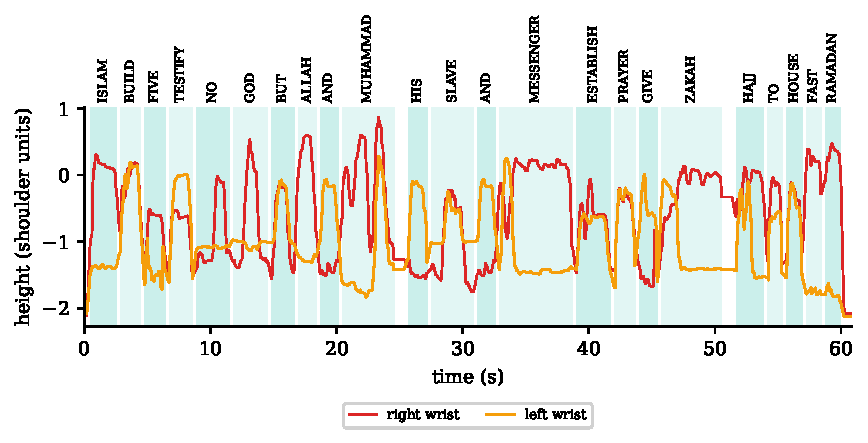
\includegraphics[width=\textwidth]{figures/timeline_en.pdf}
\caption{Concatenated pose for ``What are the pillars of Islam?'' (23 glosses, 61\,s at 25 fps): wrist height over time;
shaded bands are the sign segments, white gaps the transitions.}
\label{fig:timeline}
\end{figure}

\section{Rendering: skeleton and 3D avatar}
\label{sec:render}
\paragraph{Skeleton.} The pose is drawn on the CPU as a 512$\times$512 skeleton video (H.264, 25 fps), which always
works and shows the hands exactly as recorded (Figure~\ref{fig:skeleton}).

\begin{figure}[ht]
\centering
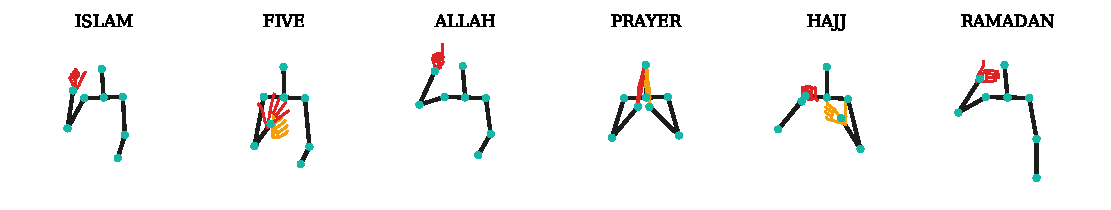
\includegraphics[width=\textwidth]{figures/skeleton_strip_en.pdf}\\[2pt]
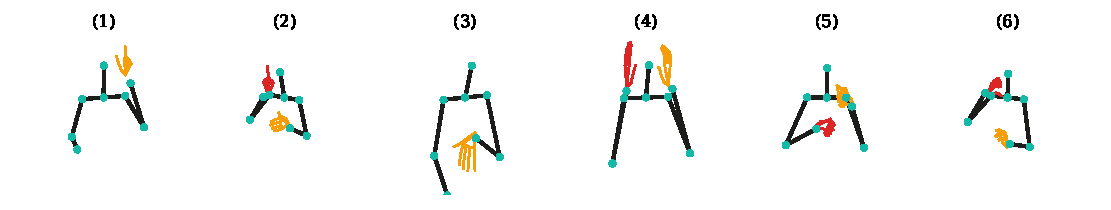
\includegraphics[width=\textwidth]{figures/skeleton_strip_ar.pdf}
\caption{Keypoints at the middle of six signs. Top: ASL (English answer). Bottom: ArSL, (1)~\ar{إسلام} (2)~\ar{الله}
(3)~\ar{محمد رسول الله} (4)~\ar{الصلاة} (5)~\ar{الزكاة} (6)~\ar{رمضان}. Teal: body joints; orange: left hand; red:
right hand.}
\label{fig:skeleton}
\end{figure}

\paragraph{Avatar.} In the browser the same pose drives a humanoid avatar in VRM format \cite{vrm}, loaded with three.js
\cite{threejs} and three-vrm \cite{threevrm}. Each arm bone is rotated so that its rest direction, measured on the avatar
in its T-pose, points along the corresponding keypoint segment; each hand takes a full orientation from two vectors
(wrist to middle knuckle, index to little knuckle), so the direction the palm faces is kept; the fingers then bend inside
the hand. MediaPipe's depth is noisy, so body depth is halved, arms are kept from passing behind the body, and rotations
are smoothed between frames (55\% of the new rotation per frame). The default model is pixiv's
\code{VRM1\_Constraint\_Twist\_Sample}, whose VRM licence allows modification, redistribution and religious and
commercial use without credit; any other VRM model placed in the application's folder can be selected.

\paragraph{Modest dress.} Outfits are built procedurally from simple shapes attached to the avatar's bones, so they
follow the signing, and they are sized from the avatar's measured face width and bone positions, so other VRM models fit
too. Three presets exist (Figure~\ref{fig:outfits}): the original clothing; a \emph{hijab} (a head cap open at the face
and a drape over neck and shoulders, with long sleeves); and a \emph{shemagh} with agal, with the model's own clothing recoloured white as a thobe. Head coverings
and sleeves are added geometry; clothing colours recolour the model's own materials. The viewer can
change the head-covering and clothing colours and the sleeves; the choice is remembered in the browser.

\begin{figure}[ht]
\centering
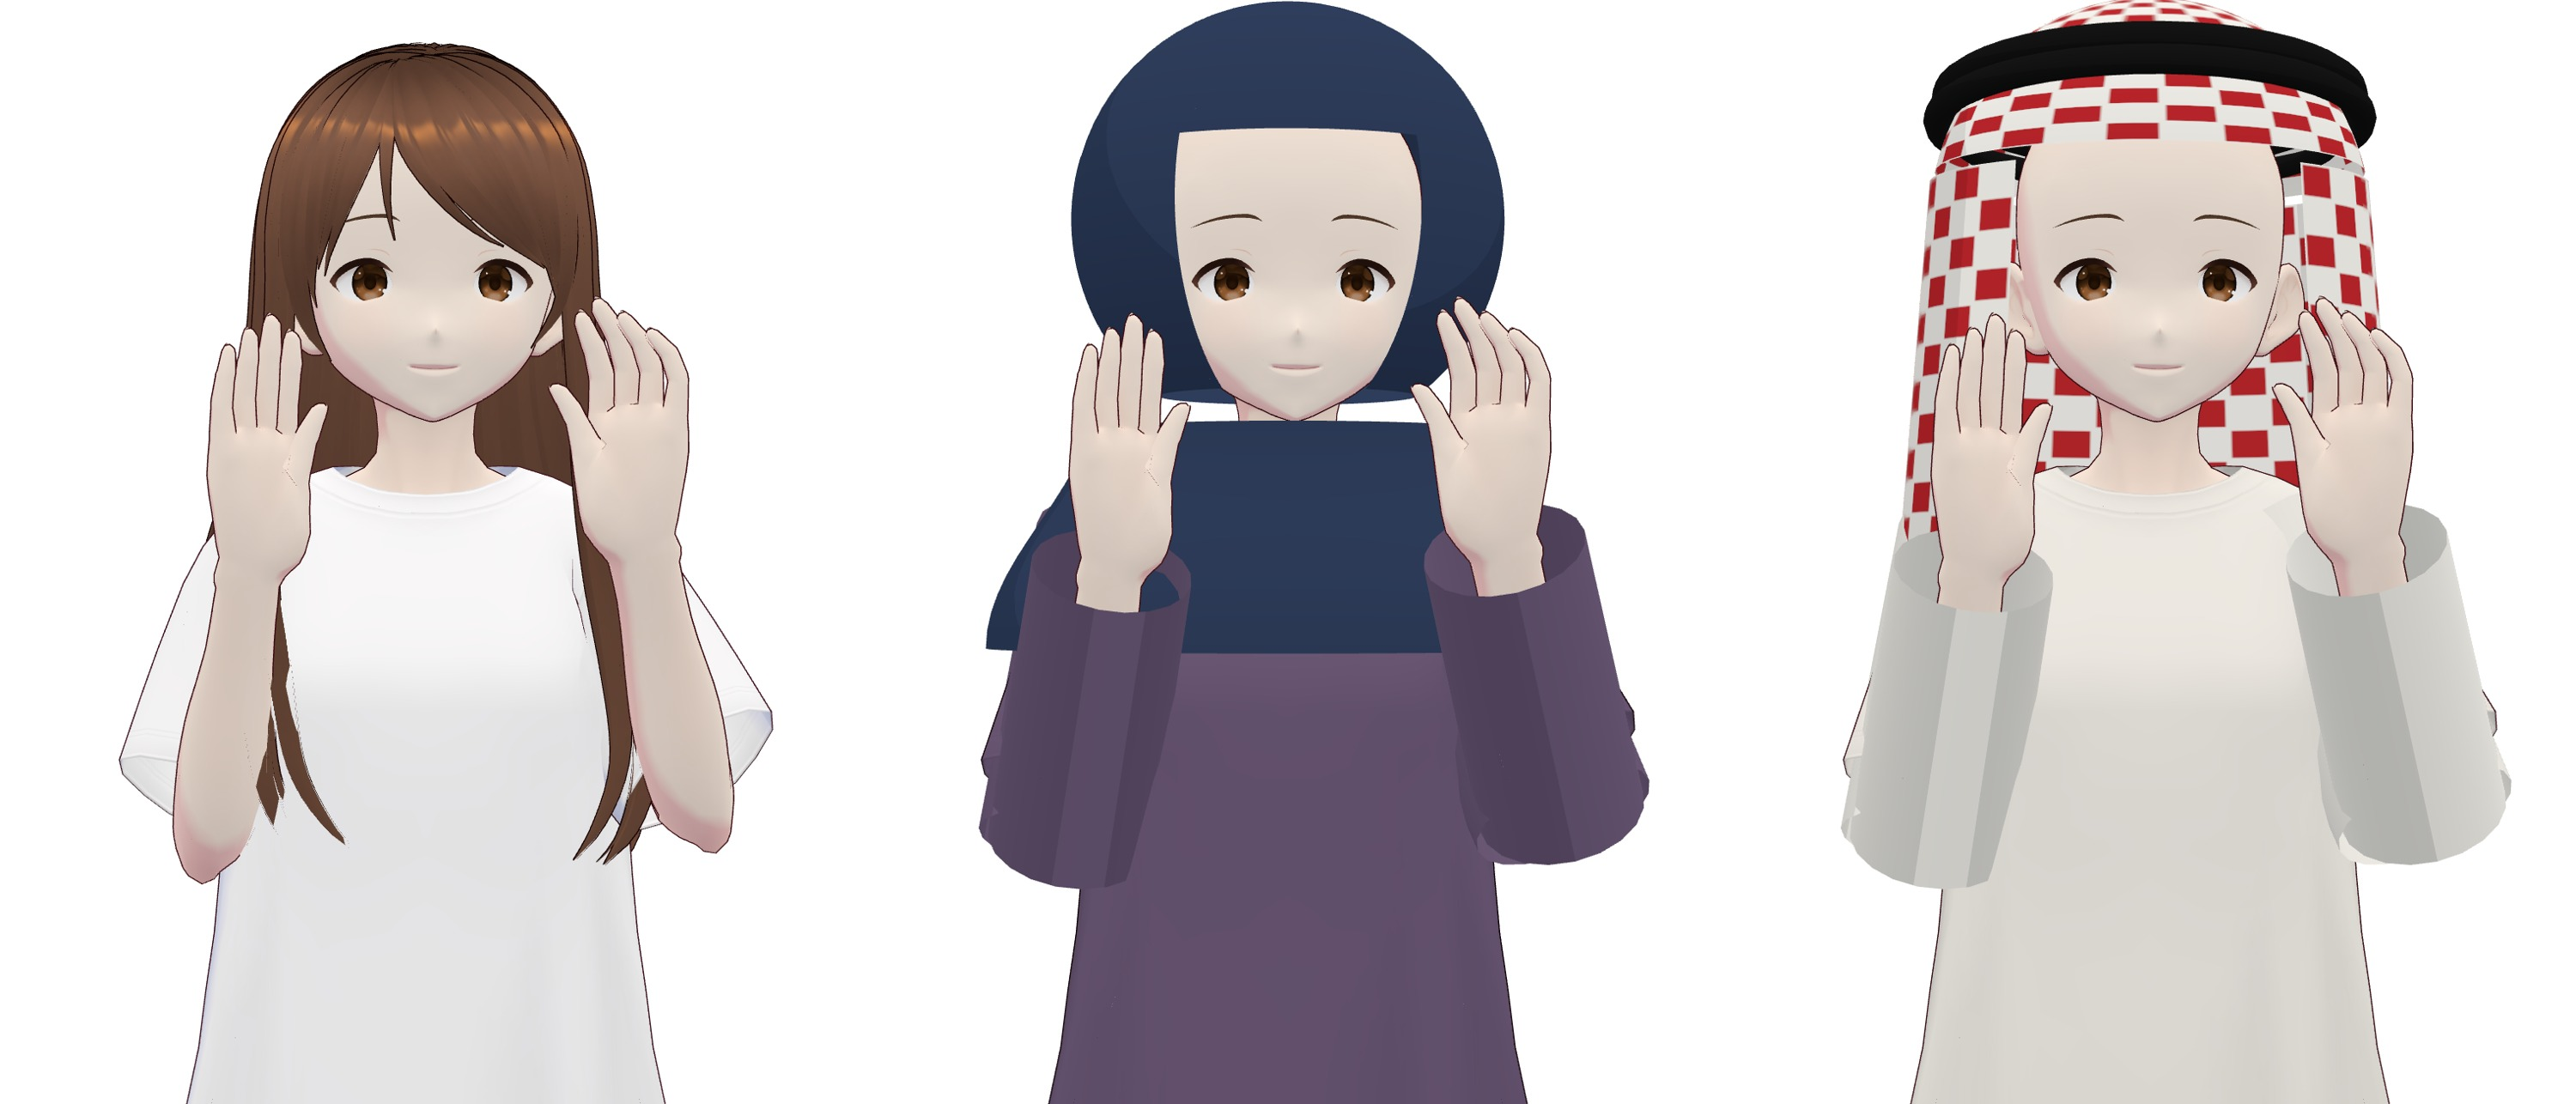
\includegraphics[width=0.78\textwidth]{figures/avatar_outfits.jpg}
\caption{The avatar presets, all signing \ar{الصلاة} (prayer) at the same frame: original, hijab, shemagh with thobe.}
\label{fig:outfits}
\end{figure}

\begin{figure}[ht]
\centering
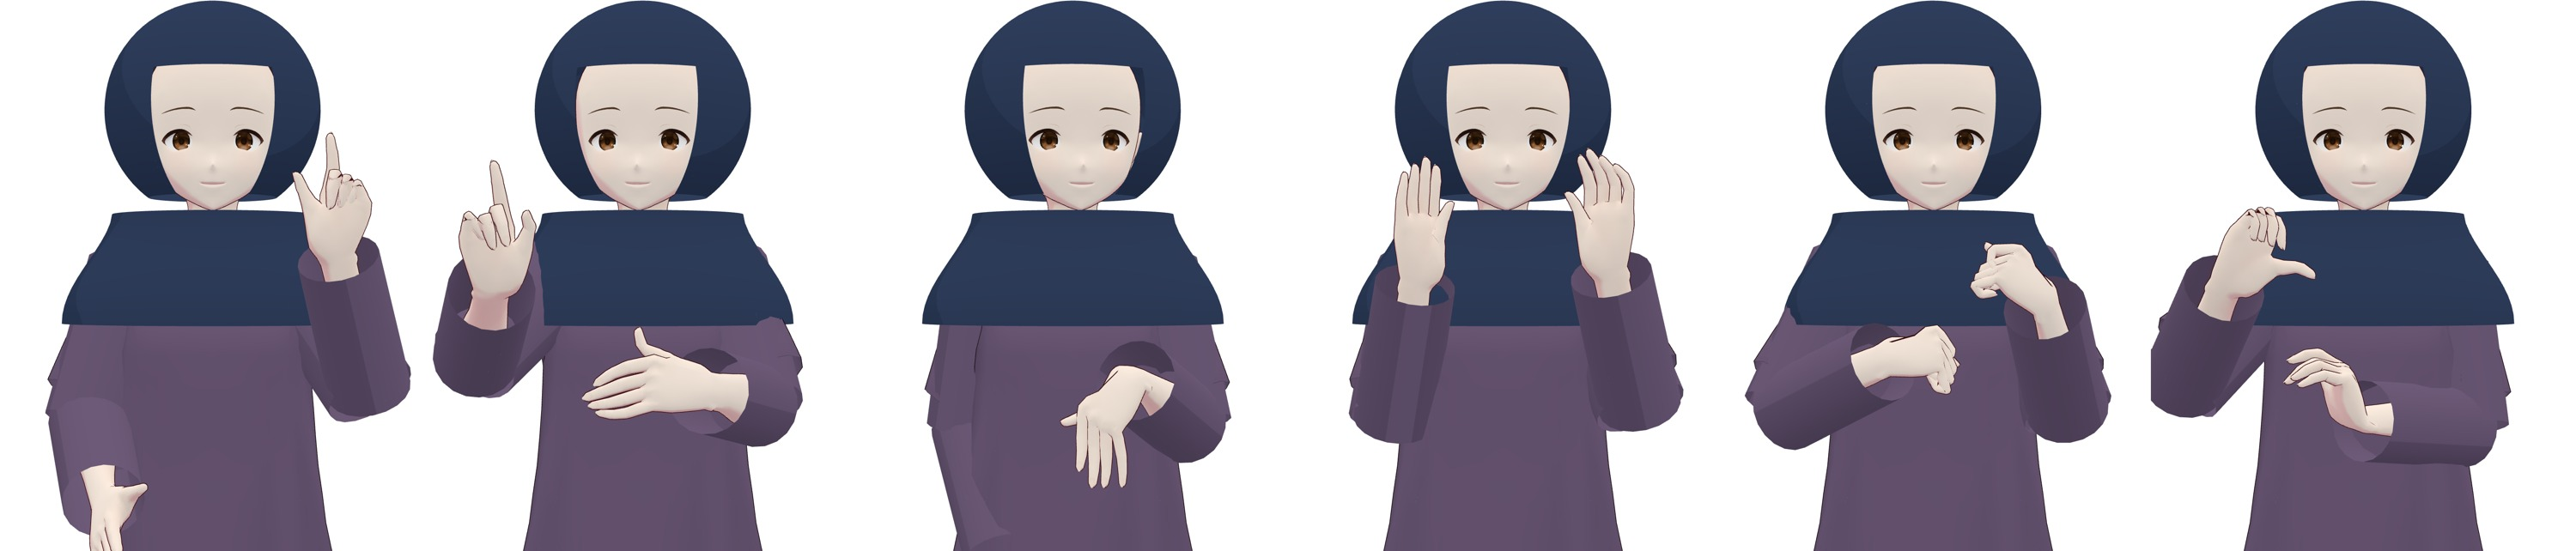
\includegraphics[width=\textwidth]{figures/avatar_strip_ar.jpg}\\[3pt]
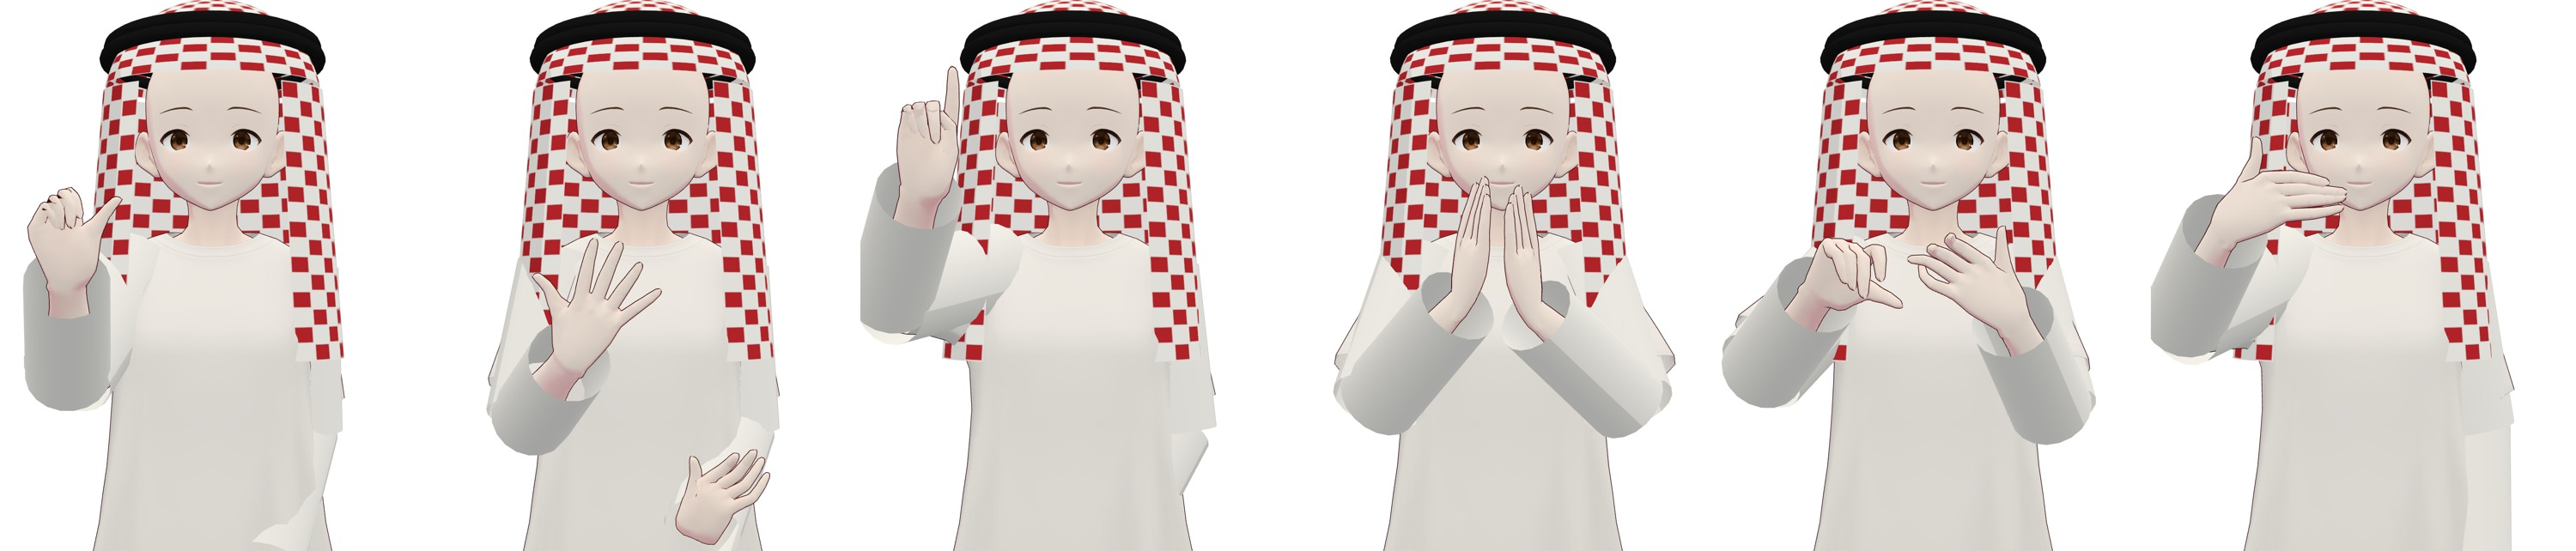
\includegraphics[width=\textwidth]{figures/avatar_strip_en.jpg}
\caption{The avatar retargeted from the generated pose. Top (hijab, ArSL): \ar{إسلام}, \ar{الله}, \ar{محمد رسول الله},
\ar{الصلاة}, \ar{الزكاة}, \ar{رمضان}. Bottom (shemagh, ASL): ISLAM, FIVE, ALLAH, PRAYER, HAJJ, RAMADAN.}
\label{fig:avatarstrip}
\end{figure}

\paragraph{Viewing controls.} Playback speed can be set to 0.5$\times$, 0.75$\times$ (default, since dictionary signs
joined back to back look fast), 1$\times$ or 1.25$\times$; the speed applies to the avatar, the skeleton and the export.
The avatar animation can be exported as a video file (MP4 where the browser supports it, otherwise WebM) at 30 fps.
